\subsection{SnaHyp parametric equation}

\begin{table}[ht]
	\begin{center}
		\begin{tabular}[top]{ |p{16.0 cm}| }
			\rowcolor{LIGHTCYAN}			
		 
			\rowcolor{LIGHTCYAN}
			\hline \textbf{No. 8 - SnaHyp = Sum of (Snailshell + Hypotrocoid) parametric curves}\\

			\begin{eqnarray}
				xsna(u) & = & [4\sin(8\pi u) ] / [16 (\pi u)^2 + 4] \nonumber \\
				xhyp(u) & = & [2\cos(4\pi u)  + 5\cos(8\pi u /3)  ] \nonumber \\
				x(u) & = & 10[xsna(u) + xhyp(u)] \nonumber \\
			    ysna(u) & = & [10\cos(8\pi u)] / [16 (\pi u)^2 + 4] \nonumber \\
				yhyp(u) & = & [2\sin(8\pi u) - 5\sin(8\pi u /3)] \nonumber \\
				y(u) & = & 10[ysna(u) + yhyp(u)] \nonumber \\
				u & \in & [0.0, 1.0] \nonumber
			\end{eqnarray}

%% double scaleup = 10.0;
%% double k = (4.0 * PI_cpos);
%% double small = 1.0e-10;
%% double x_sna = (4.0)*( sin(2*k*u) / (k*u*k*u + 4.0) );
%% double x_hyp = (2*cos(k*u) + 5*cos(2*k*u/3));
%% double x = x_sna + x_hyp;
%% return (scaleup)*(x);

%% double scaleup = 10.0;
%% double k = (4.0 * PI_cpos);
%% double small = 1.0e-10;
%% double y_sna = (10)*(cos(2*k*u) / (k*u*k*u + 4.0));
%% double y_hyp = (2*sin(k*u) - 5*sin(2*k*u/3));
%% double y = y_sna + y_hyp;
%% return (scaleup)*(y);			
			
			Open ended curve\\
			Overall 1 loop, except for 1 concave curve, the rest are convex curves \\
			Reflection x-axis: non-symmetrical\\
			Reflection y-axis: non-symmetrical\\
			\frame{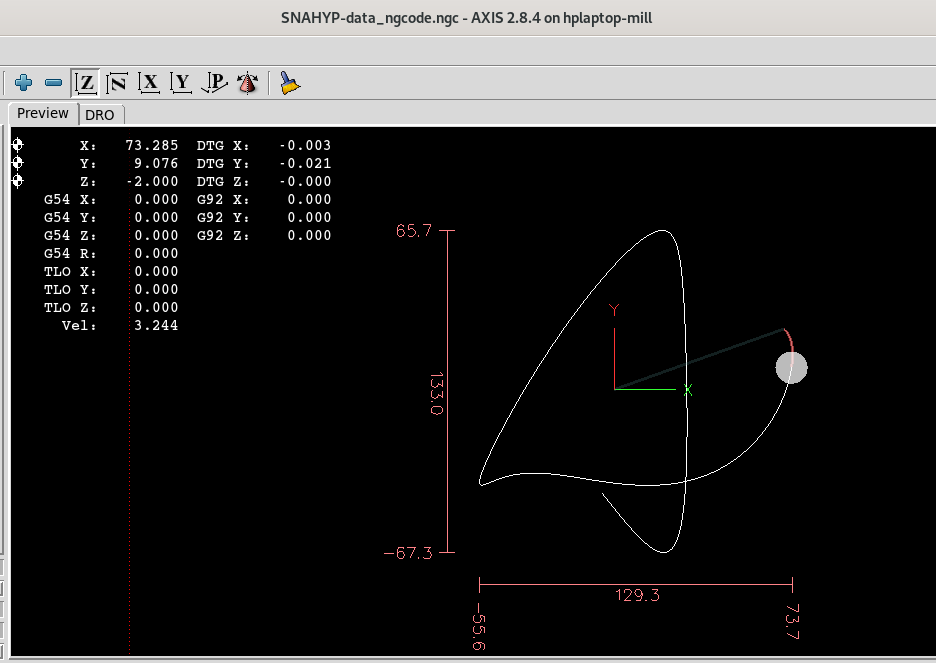
\includegraphics[width=0.560\textwidth]{./07-images/img-Ch5/SNAHYP-Axis.png}}
			\frame{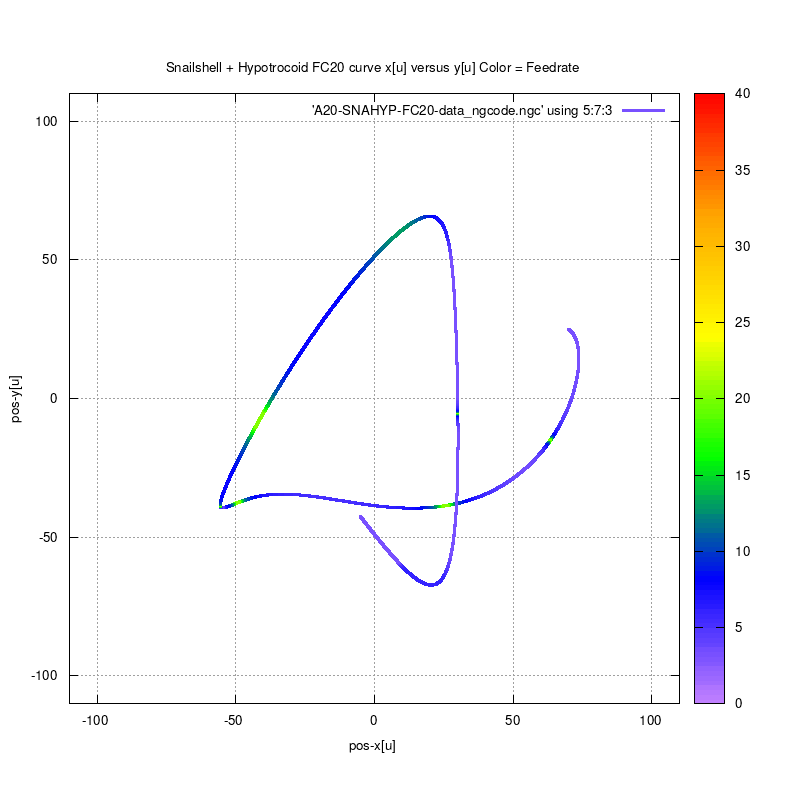
\includegraphics[width=0.395\textwidth]{./07-images/img-Ch5/SNAHYP-Feedrate.png}}\\
			
			\hline
		\end{tabular}
		\caption{SnaHyp equation and dimensions}		
		\label{table:SnaHyp equation and dimensions}
	\end{center}
\end{table}  
